\documentclass{article}
\usepackage{graphicx}
\usepackage{amsmath}
\usepackage{indentfirst}
\usepackage[brazilian]{babel}
\usepackage{hyperref}
\renewcommand{\tablename}{Tabela}
\renewcommand{\figurename}{Figura}
\title{Atividade Avaliativa de Álgebra linear}
\author{Lucas Emanoel, Rafael Emanuel, Éricles Barros \\João Pedro Ferreira, Ruslan Andruscha}
\date{25 de março de 2024}

\begin{document}

\maketitle


%primeira
\section{Escolhendo uma base de dados}
    Nossa equipe optou por utilizar o Datasheet nº2 que contém os seguintes dados:
    
    \begin{table}[ht]
        \centering
        \begin{tabular}{|c|c|c|}
        \hline
        \textbf{Pessoa} & \textbf{Peso (kg)} & \textbf{Altura (cm)} \\
        \hline
            Pessoa 1 & 52 & 158 \\
        \hline
            Pessoa 2 & 92 & 175 \\
        \hline
            Pessoa 3 & 55kg & 172cm \\
        \hline
            Pessoa 4 & 54 & 155 \\
        \hline
            Pessoa 5 & 80 & 174 \\
        \hline
            Pessoa 6 & 45kg & 150cm \\
        \hline
            Pessoa 7 & 68 & 167 \\
        \hline
            Pessoa 8 & 70 & 1.68 \\
        \hline
            Pessoa 9 & 68 & 167 \\
        \hline
            Pessoa 10 & 62 & 175 \\
        \hline
        \end{tabular}
        \caption{Dados de peso e altura das pessoas.}
        \label{tab:dados}
    \end{table}
    
    Dividimos esses dados em 2 conjuntos. O primeiro, chamado Conjunto de Treino, contém as primeiras 7 instâncias da nossa base de dados.
    
    \begin{table}[ht]
        \centering
        \begin{tabular}{|c|c|c|}
        \hline
        \textbf{Pessoa} & \textbf{Peso (kg)} & \textbf{Altura (cm)} \\
        \hline
            Pessoa 1 & 52 & 158 \\
        \hline
            Pessoa 2 & 92 & 175 \\
        \hline
            Pessoa 3 & 55kg & 172cm \\
        \hline
            Pessoa 4 & 54 & 155 \\
        \hline
            Pessoa 5 & 80 & 174 \\
        \hline
            Pessoa 6 & 45kg & 150cm \\
        \hline
            Pessoa 7 & 68 & 167 \\
        \hline
        \end{tabular}
        \caption{Conjunto de Treino.}
        \label{tab:treino}
    \end{table}
    
    \newpage
    O segundo conjunto foi nomeado como Conjunto de Teste e compreende as últimas 3 instâncias da nossa base de dados:
    \begin{table}[ht]
        \centering
        \begin{tabular}{|c|c|c|}
        \hline
        \textbf{Pessoa} & \textbf{Peso (kg)} & \textbf{Altura (cm)} \\
        \hline
            Pessoa 8 & 70 & 1.68 \\
            Pessoa 9 & 68 & 167 \\
            Pessoa 10 & 62 & 175 \\
        \hline
        \end{tabular}
        \caption{Conjunto de Teste.}
        \label{tab:treino}
    \end{table}


% segunda
\section{Tratando a base de dados}
    Visando igualar a natureza dos dados que vamos manipular, trataremos o peso e altura como valores inteiros, eliminando informações irrelevantes e padronizando suas unidades. A nova base de dados terá a seguinte forma:
    
    \begin{table}[h]
        \centering
        \begin{tabular}{|c|c|c|}
        \hline
        \textbf{Pessoa} & \textbf{Peso (kg)} & \textbf{Altura (cm)} \\
        \hline
            Pessoa 1 & 52 & 158 \\
        \hline
            Pessoa 2 & 92 & 175 \\
        \hline
            Pessoa 3 & 55 & 172 \\
        \hline
            Pessoa 4 & 54 & 155 \\
        \hline
            Pessoa 5 & 80 & 174 \\
        \hline
            Pessoa 6 & 45 & 150 \\
        \hline
            Pessoa 7 & 68 & 167 \\
        \hline
            Pessoa 8 & 70 & 168 \\
        \hline
            Pessoa 9 & 68 & 167 \\
        \hline
            Pessoa 10 & 62 & 175 \\
        \hline
        \end{tabular}
        \caption{Dados de peso e altura após o tratamento}
        \label{tab:dados}
    \end{table}

    Essa simples manipulação é extremamente poderosa e permite que possamos escrever o Conjunto de treino como sendo: \\
    \begin{table}[ht]
        \centering
        \begin{tabular}{|c|c|c|}
        \hline
        \textbf{Pessoa} & \textbf{Peso (kg)} & \textbf{Altura (cm)} \\
        \hline
            Pessoa 1 & 52a & 158 \\
        \hline
            Pessoa 2 & 92a & 175 \\
        \hline
            Pessoa 3 & 55a & 172 \\
        \hline
            Pessoa 4 & 54a & 155 \\
        \hline
            Pessoa 5 & 80a & 174 \\
        \hline
            Pessoa 6 & 45a & 150 \\
        \hline
            Pessoa 7 & 68a & 167 \\
        \hline
        \end{tabular}
        \caption{Conjunto de Treino.}
        \label{tab:treino}
    \end{table}
    
    Como veremos a seguir, esse formato será muito útil e posteriormente permitirá a formação de um sistema linear preditivo.
    
% terceira
\section{Obtendo um sistema linear}
    Se considerarmos a coluna de pesos como valores de x e a
    coluna das alturas como valores de y, podemos obter o seguinte sistema linear:
    \begin{center}
        1. \quad 52a + b = 158 \\
        2. \quad 92a + b = 175 \\
        3. \quad 55a + b = 172 \\
        4. \quad 54a + b = 155 \\
        5. \quad 80a + b = 174 \\
        6. \quad 45a + b = 150 \\
        7. \quad 68a + b = 167 \\
    \end{center}


% quarta
\section{Sistema no Formato Matricial}
    Podemos reescrever o sistema linear anterior no formato matricial. Assim, nosso sistema adquire a forma:
    \[
    \begin{bmatrix}
        52 & 1 \\
        92 & 1 \\
        55 & 1 \\
        54 & 1 \\
        80 & 1 \\
        45 & 1 \\
        68 & 1 \\
    \end{bmatrix}
    .
    \begin{bmatrix}
        a \\
        b \\
    \end{bmatrix}
    =
    \begin{bmatrix}
        158 \\
        175 \\
        172 \\
        155 \\
        174 \\
        150 \\
        167 \\
    \end{bmatrix}
    \]
    
    Onde a primeira matriz é chamada de matriz dos coeficientes, a segunda de matriz das incógnitas e a terceira de matriz dos termos independentes.


% quinta
\section{Atribuindo Nomes e Tratando o Sistema}

    Adotaremos A para referir-se à matriz dos coeficientes, X para referir-se à matriz das incógnitas e Y para referir-se à matriz dos termos independentes.
    Com isso, temos que:
    \newline
    \begin{align*}
        \begin{minipage}{.3\textwidth}
            \[ A = \begin{bmatrix}
            52 & 1 \\
            92 & 1 \\
            55 & 1 \\
            54 & 1 \\
            80 & 1 \\
            45 & 1 \\
            68 & 1 \\
            \end{bmatrix} \]
        \end{minipage}
        &
            \begin{minipage}{.3\textwidth}
            \[ X = \begin{bmatrix}
                a \\
                b \\
            \end{bmatrix} \]
        \end{minipage}
        &
        \begin{minipage}{.3\textwidth}
            \[ Y = \begin{bmatrix}
                158 \\
                175 \\
                172 \\
                155 \\
                174 \\
                150 \\
                167 \\
            \end{bmatrix} \]
        \end{minipage}
    \end{align*}
    \newpage
    
    Queremos $A^\top A$ e $A^\top Y$. Para tal, calcularemos primeiramente $A^\top$.
    \begin{center}
        $A^\top = 
        \begin{bmatrix}
            52 & 92 & 55 & 54 & 80 & 45 & 68 \\
            1 & 1 & 1 & 1 & 1 & 1 & 1 \\
        \end{bmatrix}$
    \end{center}
    
    Logo, $A^\top A$ trata-se da matriz:
    \begin{center}
        $A^\top A$ =
        $\begin{bmatrix}
            52 & 92 & 55 & 54 & 80 & 45 & 68 \\
            1 & 1 & 1 & 1 & 1 & 1 & 1 \\
        \end{bmatrix}
        \cdot
        \begin{bmatrix}
            52 & 1 \\
            92 & 1 \\
            55 & 1 \\
            54 & 1 \\
            80 & 1 \\
            45 & 1 \\
            68 & 1 \\
        \end{bmatrix}
        =
            \begin{bmatrix}
            30158 & 446 \\
            446 & 1 \\
        \end{bmatrix}$
    \end{center}

    Podemos também calcular $A^\top Y$:
    \begin{center}
        $A^\top Y$ = 
        $\begin{bmatrix}
            52 & 92 & 55 & 54 & 80 & 45 & 68 \\
            1 & 1 & 1 & 1 & 1 & 1 & 1 \\
        \end{bmatrix}
        \cdot
        \begin{bmatrix}
            158 \\
            175 \\
            172 \\
            155 \\
            174 \\
            150 \\
            167 \\
        \end{bmatrix}
        =
        \begin{bmatrix}
            74172 \\
            1151 \\
        \end{bmatrix}$
    \end{center}


% sexta
\section{Encontrando a Solução do SL $A^\top AX$ = $A^\top Y$}
    \begin{center}
        $\begin{bmatrix}
        30158 & 446 \\
        446 & 1 \\
        \end{bmatrix}
        .
        \begin{bmatrix}
        a & b \\
        \end{bmatrix}
        =
        \begin{bmatrix}
        74172 \\
        1151 \\
        \end{bmatrix}$
    \end{center}
    \begin{align}
        &30158\textit{a} + 446\textit{b} = 74172 \\
        &446\textit{a} + \textit{b} = 1151
    \end{align}
    
    A partir de (2) temos:
    \begin{align}
        &\textit{b} = 1151 - 446\textit{a}
    \end{align}
    
    Substituindo(3) em (1), temos:
    \begin{center}
        \begin{align*}
            &30158\textit{a} + 446(1151 - 446\textit{a}) = 74172 \\
            &30158\textit{a} + 513346 - 198916\textit{a} = 74172 \\
            &-168758\textit{a} = 74172 - 513346 \\
            &168758\textit{a} = 439174       
        \end{align*}
        \begin{align}
            \textit{a} \approx 2,6
        \end{align}
    \end{center}
    \newpage
    
    Obtendo o valor de \textit{a} podemos substituir (4) em (2):
    \begin{center}
        \begin{align*}
            &446\textit{a} + \textit{b} = 1151 \\
            &1159,6 + \textit{b} = 1151
        \end{align*}
            \begin{align}
                &\textit{b} = -8,6
            \end{align}
    \end{center}
    

% setima
\section{Encontrando a Equação da Reta}
    No item anterior, descobrimos os valores dos coeficientes \textit{a} e \textit{b}
    \begin{align*}
        \textit{a} \approx 2,6 \\
        \textit{b} = -8,6
    \end{align*}        
    
    Temos que a forma geral da equação de uma reta é dado por
    \begin{align}
        \textit{y} = \textit{ax} + \textit{b}
    \end{align}

    Substituindo (3) e (4) em (6) é possível encontrar a equação da reta que melhor descreve o comportamento do nosso sistema linear:
    \begin{align}
        \textit{r}: 2,6\textit{x} - 8,6
    \end{align}
    
    A próxima etapa consiste em utilizar o Conjunto de Teste para quantificar a precisão do nosso modelo.
    \begin{table}[ht]
    \centering
    \begin{tabular}{|c|c|c|}
    \hline
    \textbf{Pessoa} & \textbf{Peso (kg)} & \textbf{Altura (cm)} \\
    \hline
        Pessoa 8 & 70 & 168 \\
    \hline
        Pessoa 9 & 68 & 167 \\
    \hline
        Pessoa 10 & 62 & 175 \\
    \hline
    \end{tabular}
    \caption{Conjunto de Teste.}
    \label{tab:treino}
    \end{table}


% oitava
\section{Teste do Modelo Linear}
    Utilizando os dados contidos no Conjunto de Teste, é possível realizar previsões baseadas no comportamento da equação linear encontrada no item anterior.
    
    Tais previsões podem não apresentar o real valor da altura do indivíduo, mas deve representar uma boa aproximação desde que o erro relativo esteja contido no intervalo esperado.
    
    É possível calcular o erro relativo utilizando a seguinte expressão:
    \begin{center}
        $Erro\textsubscript{relativo} = \frac{Medida\textsubscript{real} - Medida\textsubscript{prevista}}{Medida\textsubscript{real}} \times 100\%$ \\
    \end{center}
    \newpage
    
    Em posse dessa equação e com um modelo de previsão, foi possível gerar os seguintes dados: 
    \begin{center}
        \begin{table}[ht]
        \begin{tabular}{|c|c|c|c|c|}
        \hline
        \textbf{Nome} & \textbf{Peso (kg)} & \textbf{Altura (cm)} & \textbf{Prev. do Modelo (cm)} & \textbf{Erro Relativo} \\
        \hline
            Pessoa 8 & 70 & 168  & 173,4 & 3,21\% \\
        \hline
            Pessoa 9 & 68 & 167  & 168,2 & 0,84\% \\
        \hline
            Pessoa 10 & 62 & 175 & 152,6 & 12,80\% \\
        \hline
        \end{tabular}
            \caption{Previsão do Modelo}
        \label{tab:treino}
        \end{table}
    \end{center}

\section{Enriquecendo nosso Modelo}
    O objetivo desse item é analisar a correlação entre os dados que estamos estudando, além de finalmente adentrar no âmbito computacional e de fato analisar o funcionamento do modelo.
    
    Dentre as tecnologias aptas a desenvolver essa atividade, a equipe optou por utilizar-se da linguagem de programação Python. Utilizamos a biblioteca pandas para manipular a base de dados, matplotlib para plotar o gráfico de dispersão e numpy para calcular o coeficiente de correlação entre os dados do nosso sistema. O código gerado pode ser encontrado no repositório público \textbf{\href{https://github.com/lucaasifx/atividadeAlgebra}{atividadeAlgebra}}.

    O coeficiente de correlação $\rho$ pode assumir valores entre -1 e 1, onde:
    \begin{align*}
        \rho &= 0,9 \text{ a } 1 \quad (\text{positivo ou negativo}): \text{correlação muito forte}; \\
        \rho &= 0,7 \text{ a } 0,9 \quad (\text{positivo ou negativo}): \text{correlação forte}; \\
        \rho &= 0,5 \text{ a } 0,7 \quad (\text{positivo ou negativo}): \text{correlação moderada}; \\
        \rho &= 0,3 \text{ a } 0,5 \quad (\text{positivo ou negativo}): \text{correlação fraca}; \\
        \rho &= 0 \text{ a } 0,3 \quad (\text{positivo ou negativo}): \text{não possui correlação}.
    \end{align*}

    Utilizando o método corrcoef contido na biblioteca numpy, foi possível verificar que o $\rho$ da nossa base de dados é dado por:
    \begin{align*}
        \rho = 0,742
    \end{align*}

    Esse valor é expressivo e indica que os nossos dados possuem uma forte correlação entre si.

    O próximo passo foi plotar o gráfico de dispersão dos dados. Para isso, foram utilizadas diversas ferramentas da biblioteca matplotlib. O resultado pode ser visualizado abaixo:
    \newpage
    \begin{center}
        \begin{figure}[ht]
            \centering
            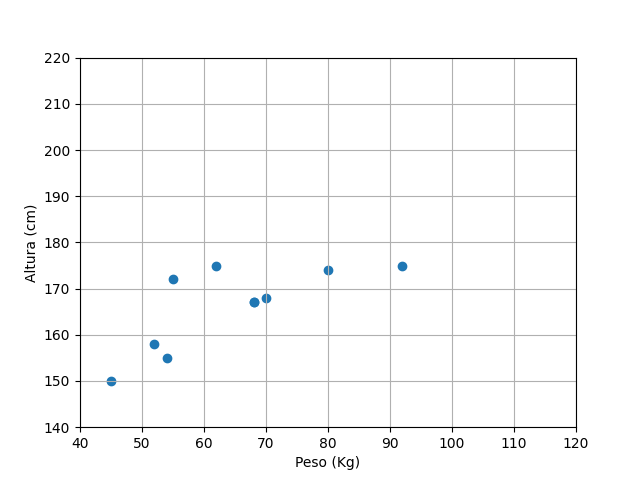
\includegraphics[width=0.6\textwidth]{Figure_1.png}
            \caption{Gráfico de dispersão do Datasheet 2}
            \label{fig:enter-label}
        \end{figure}
    \end{center}
    
    Verificamos também que essa seria uma excelente oportunidade para testar o modelo de previsão que vínhamos desenvolvendo durante toda a atividade. Adicionalmente ao gráfico de dispersão, plotamos a equação (7), obtendo o gráfico à seguir:
    \begin{center}
        \begin{figure}[ht]
            \centering
            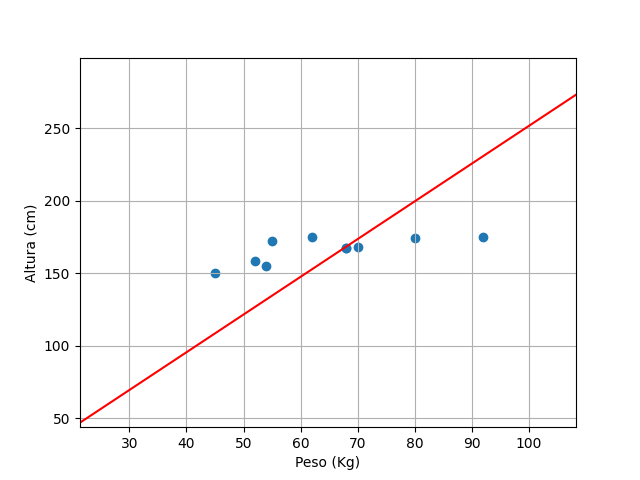
\includegraphics[width=0.6\textwidth]{Figure_2.png}
            \caption{Reta \textit{r}: 2,6\textit{x} - 8,6 aplicada ao gráfico de dispersão}
            \label{fig:enter-label}
        \end{figure}
    \end{center}

    Com isso, podemos concluir que o nosso modelo apresenta uma aproximação satisfatória dos resultados reais esperados.


\section{Considerações Finais}
    Após completar a atividade avaliativa de Álgebra Linear, nossa equipe alcançou diversas conclusões significativas. Primeiramente, ficou claro como os conceitos de Álgebra Linear são fundamentais e aplicáveis em contextos do mundo real, como a modelagem de dados de peso e altura. Através da construção de um sistema linear e da resolução matricial, pudemos compreender como esses conceitos são essenciais na formulação e resolução de problemas complexos.

    Além disso, a atividade nos permitiu aplicar esses conceitos utilizando ferramentas computacionais modernas, como Python, o que reforçou a importância da programação na análise e interpretação de dados. Através da manipulação e visualização dos dados, pudemos entender melhor o relacionamento entre as variáveis e avaliar a qualidade do modelo linear proposto.
\end{document}
